\documentclass{ctpro}
\usepackage{shortvrb}

\title{ACM算法与微应用实验室2021年11月月赛题目}
\date{2021年12月1日}

\begin{document}
\maketitle
\addproblem{克隆干员}{1000}{128}{传统}{AgOH}
\addproblem{中转站}{1000}{128}{传统}{AgOH\&Tifa}
\addproblem{三斜求积术}{1000}{128}{传统}{AgOH}
\addproblem{子树大小}{1000}{128}{传统}{AgOH}
\addproblem{雷立方体阵列}{1500}{64}{传统}{Tifa}
\addproblem{Go}{1000}{128}{传统}{AgOH}

\section*{比赛信息}
\ctinfotab{ACM\ |个人赛|不封榜}{C/C++,Python,Java}{3}

\section*{题目概况}
\problemtab

\section*{编译命令}
参见OJ帮助

\section*{注意事项}
\begin{itemize}
	\item C/C++中函数main()的返回值类型必须是int,程序正常结束时的返回值必须是0。
	\item C/C++代码必须完全符合GNU C/C++ 标准,不能使用诸如绘图、Win32API、中断调用、硬件操作或与操作系统相关的API。
	\item C/C++代码中允许使用STL类库。
\end{itemize}

\paragraph*{} 祝大家取得好成绩!

\MakeShortVerb{\|}
\makeproblem
\section*{题目描述}
不久前,明日方舟中添加了克隆干员的新玩法(误),|AgOH|迫不及待地想要尝试一下。

进入战场后|AgOH|瞬间就放下了好几个\textbf{同一名}干员,而且因为|AgOH|手抖,各干员的朝向并不完全相同,正当|AgOH|窃喜之时,他发现了一个严重的问题:干员的攻击范围显示不知为何消失了。

|AgOH|知道这名干员的攻击范围是多大,但因为|AgOH|太菜了,他想不出多个这名干员同时在场时的总攻击范围是什么样子的,你能帮帮他吗?

注:战场为一个 $10 \times 10$ 的矩形。

\section*{输入格式}
首先,一个 $7 \times 7$ 的矩形,表示这名干员\textbf{站在矩形中点 $(4,4)$ 并朝上}时的攻击范围。矩形中能被干员攻击到的位置用|1|表示,不能被干员攻击到的位置用|0|表示。

接下来一行,一个整数 $n~(1 \leq n \leq 10)$,代表|AgOH|放下了多少个这名干员。

接下来 $n$ 行,每行三个整数 $x,y,f~(1 \leq x,y \leq 10;~1 \leq f \leq 4)$,分别代表干员所站的位置 $(x,y)$ 及朝向。$f=1,2,3,4$ 时干员分别朝向上、下、左、右。

\section*{输出格式}
一个 $10 \times 10$ 的矩形,其中能被干员攻击到的位置用|1|表示,不能被干员攻击到的位置用|0|表示。

\section*{输入输出样例}
\testcasetab
{
	0001000\par
	0001000\par
	0011100\par
	0011100\par
	0000000\par
	0000000\par
	0000000\par
	4\par
	1 1 4\par
	5 5 2\par
	4 6 3\par
	8 7 1
}
{
	1111000000\par
	1100000000\par
	0000110000\par
	0011110000\par
	0001111000\par
	0001111000\par
	0000111100\par
	0000111100\par
	0000000000\par
	0000000000
}

\section*{说明/提示}
【样例解释】

4个这个干员放下后,战场情况如图所示:

\begin{center}
	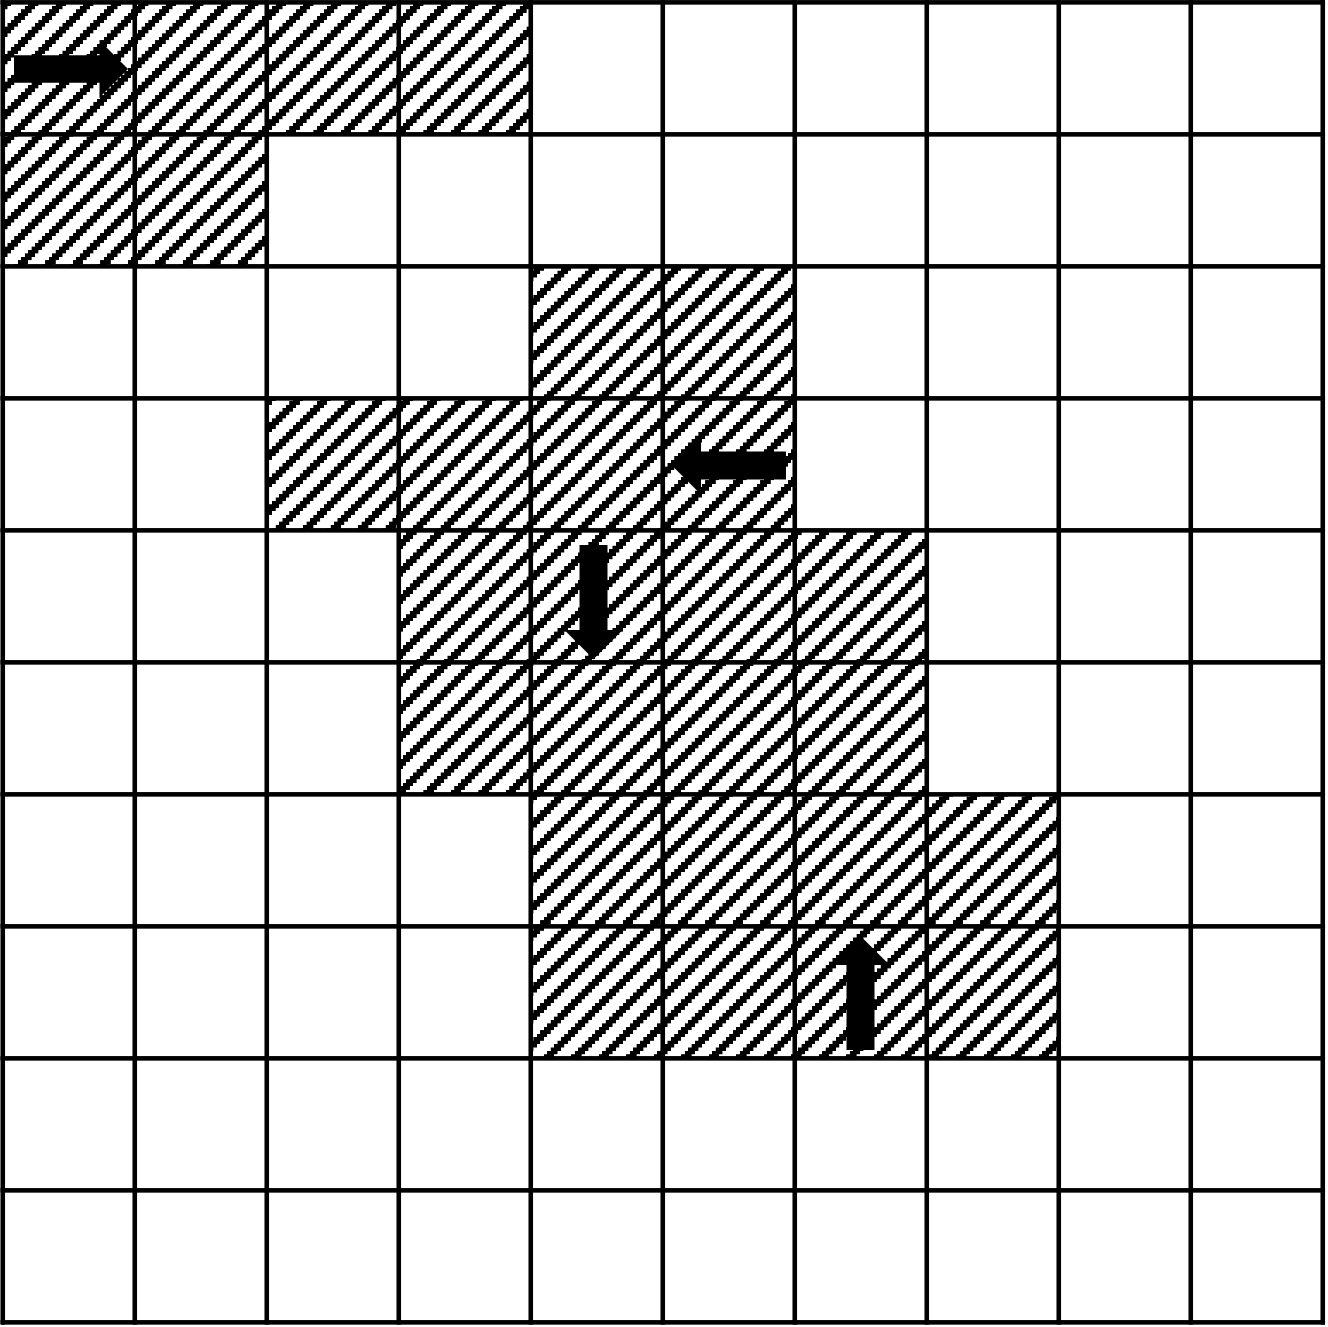
\includegraphics{images/battlefield.png}
\end{center}

\makeproblem
\section*{题目描述}
小Z发明了一个游戏,内容是这样的:玩家一开始站在A点,目标是去往B点,但A点与B点之间并没有直达线路,必须要从C点中转。从A点到C点共有 $n$ 条线路可供选择,每条线路的分数分别为 $a_1, a_2, \cdots, a_n$;从C点到B点也有 $n$ 条线路可供选择,每条线路的分数分别为 $b_1, b_2, \cdots, b_n$。若玩家采取线路 $a_i, b_j$ 来到达C点,他将获得 $a_i \times b_j$ 分。整个游戏的总分为玩家走所有可行的路线能获得的分数的和(即 $\sum_{i=1}^n \sum_{j=1}^n a_i b_j$)。

小Z自己试玩了几局后很快就厌倦了,因为他发现每次玩游戏得到的分数都是一样的,一点趣味都没有,于是他找到|Tifa|,询问能否让这个游戏每次获得的分数都不一样。|Tifa|在思索了 $1 \mu s$后想到了改进方式:规定一个区间 $[l,r]~(1 \leq l \leq r)$,并限制玩家只可以走线路 $a_l, a_{l+1}, \cdots, a_r$ 以及线路 $b_l, b_{l+1}, \cdots, b_r$,这样随着规定区间的不同,玩家所能获得的分数也就不一样了。

小Z非常高兴,他马上就想把自己的这个游戏推广出去,他找到了你并让你玩这个游戏。为了让你多玩几局,小Z让你计算出在所有可能的区间约束下,每次你能获得的分数的总和。他觉得你只有玩很多很多局游戏后才能计算出他想要的结果,得意地离开了。

现在请你计算出正确答案,并回答小Z。因为答案可能过大,你只需要输出答案对 $10^9 + 7$ 取模的结果即可。

\section*{输入格式}
第一行,一个整数 $n~(3 \leq n \leq 5 \times 10^5)$。

第二行,$n$ 个整数,代表 $a_i~(1 \leq a_i \leq 10^9)$。

第三行,$n$ 个整数,代表 $b_i~(1 \leq b_i \leq 10^9)$。

\section*{输出格式}
一行,一个整数,代表结果。

\section*{输入输出样例}
\testcasetab
{
	2\par
	1 2\par
	3 4
}
{
	32
}

\testcasetab
{
	5\par
	1 2 3 4 5\par
	5 4 3 2 1
}
{
	889
}

\section*{说明/提示}
【样例解释】

在样例1中:

若|Tifa|限制的区间为 $[1,1]$,那么小Z可以采取的线路有:

$$A \stackrel{a_1}{\rightarrow} C \stackrel{b_1}{\rightarrow} B,~score=a_1 \times b_1=3$$

他共可以获得 $3$ 分。

若|Tifa|限制的区间为 $[1,2]$,那么小Z可以采取的线路有:

$$A \stackrel{a_1}{\rightarrow} C \stackrel{b_1}{\rightarrow} B,~score=a_1 \times b_1=3$$

$$A \stackrel{a_1}{\rightarrow} C \stackrel{b_2}{\rightarrow} B,~score=a_1 \times b_2=4$$

$$A \stackrel{a_2}{\rightarrow} C \stackrel{b_1}{\rightarrow} B,~score=a_2 \times b_1=6$$

$$A \stackrel{a_2}{\rightarrow} C \stackrel{b_2}{\rightarrow} B,~score=a_2 \times b_2=8$$

他共可以获得 $3+4+6+8=21$ 分。

若|Tifa|限制的区间为 $[2,2]$,那么小Z可以采取的线路有:

$$A \stackrel{a_2}{\rightarrow} C \stackrel{b_2}{\rightarrow} B,~score=a_2 \times b_2=8$$

他共可以获得 $8$ 分。

故答案为 $3+21+8=32$。

\makeproblem
\section*{题目描述}
给出一个三角形三条边的边长,请算出这个三角形的面积。

\section*{输入格式}
第一行,一个整数 $t~(1 \leq t \leq 10^5)$,代表共有 $t$ 组数据。

对于每组数据:

\indent \indent 一行,三个整数 $a,b,c~(1 \leq a,b,c \leq 10^4)$,代表三角形三条边的长度。

\section*{输出格式}
对于每组数据,在一行内输出一个实数(四舍五入保留 $2$ 位小数),代表答案。


\section*{输入输出样例}
\testcasetab
{
	3 \par
	3 3 3\par
	3 4 5\par
	2 3 3
}
{
	3.90\par
	6.00\par
	2.83\par
}

\section*{说明/提示}
\textbf{海伦公式}
\begin{quotation}
	海伦公式又译作希伦公式、海龙公式、希罗公式、海伦-秦九韶公式。它是利用三角形的三条边的边长直接求三角形面积的公式。

	假设在平面内,有一个三角形,边长分别为 $a,b,c$,三角形的面积 $S$ 可由以下公式求得:

	$$S=\sqrt{p(p-a)(p-b)(p-c)}$$

	其中 $p$ 为三角形的半周长(周长的一半):

	$$p=\cfrac{a+b+c}{2}$$
\end{quotation}

\makeproblem
\section*{题目描述}
对于一棵树,有定义如下:

\begin{definition}[树的大小]
	树中存在的结点的数量叫做这棵树的大小。
\end{definition}

给定一棵树,请分别计算出以各结点作为根结点时各子树的大小。

\section*{输入格式}
第一行,两个整数 $n~(1 \leq n \leq 10^4)$,代表给定的树的大小。

接下来的 $n-1$ 行,每行两个整数 $u,v~(1 \leq u,v \leq n)$,代表结点 $u$ 与结点 $v$ 之间有一条边。

\section*{输出格式}
输出共 $n$ 行,每行 $n$ 个整数 $s_1,s_2,\cdots,s_n$。$s_i$ 代表以 $i$ 为根结点的子树的大小。

\section*{输入输出样例}
\testcasetab
{
	5\par
	1 2\par
	1 3\par
	2 4\par
	2 5
}
{
	5 3 1 1 1\par
	2 5 1 1 1\par
	4 3 5 1 1\par
	2 4 1 5 1\par
	2 4 1 1 5
}

\section*{说明/提示}
【样例解释】

分别以 $1 \sim 5$ 号结点作为根结点时,各子树大小:
\begin{figure}
	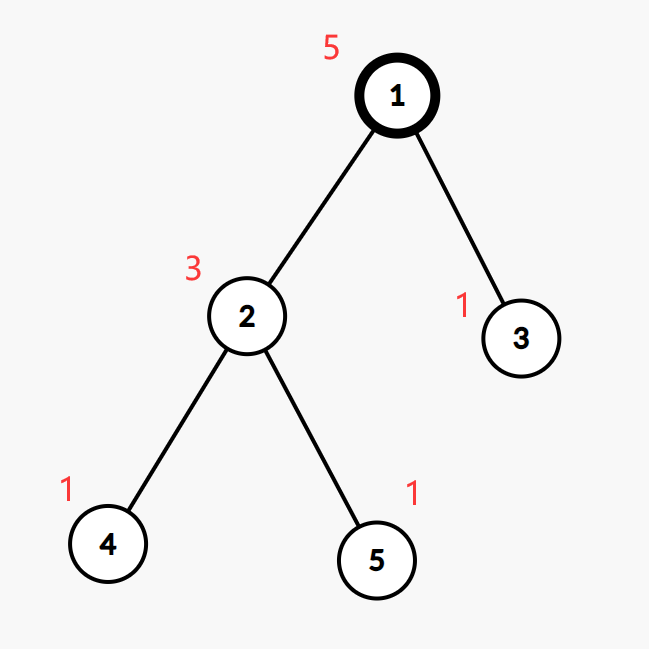
\includegraphics[scale=0.14]{images/D_1.png}
	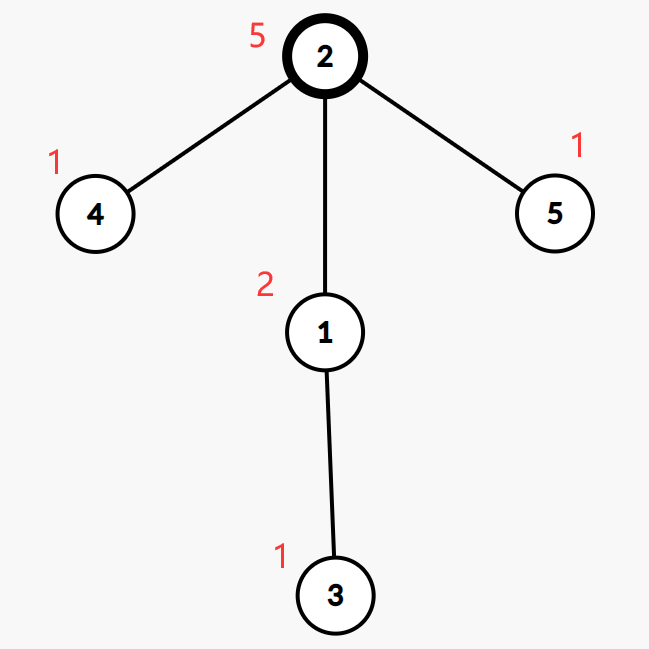
\includegraphics[scale=0.14]{images/D_2.png}
	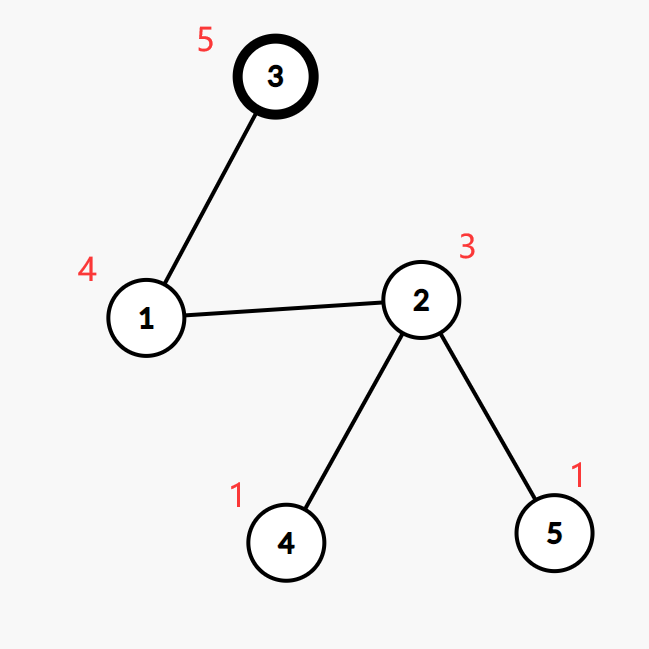
\includegraphics[scale=0.14]{images/D_3.png}
	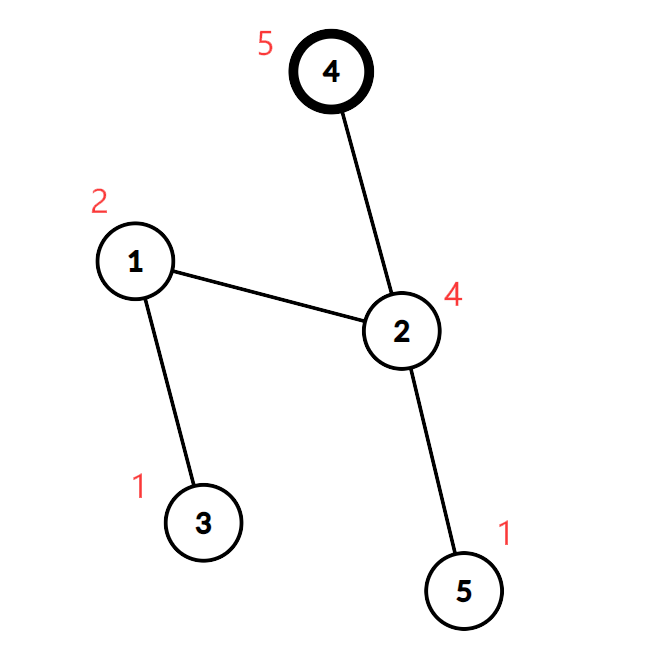
\includegraphics[scale=0.14]{images/D_4.png}
	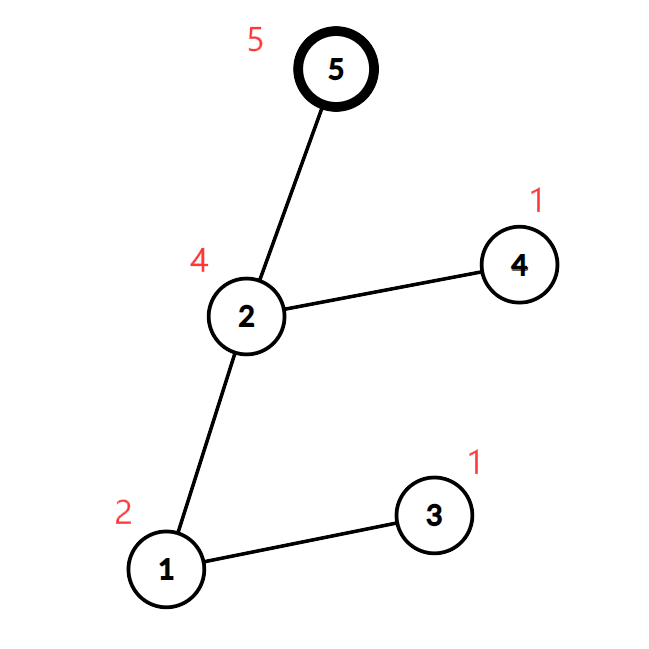
\includegraphics[scale=0.14]{images/D_5.png}
\end{figure}

\makeproblem
\section*{题目描述}

|Tifa| 在提瓦特世界里发现了一个奇妙的机关:雷立方体。

\vspace{0.2em}

\begin{center}
    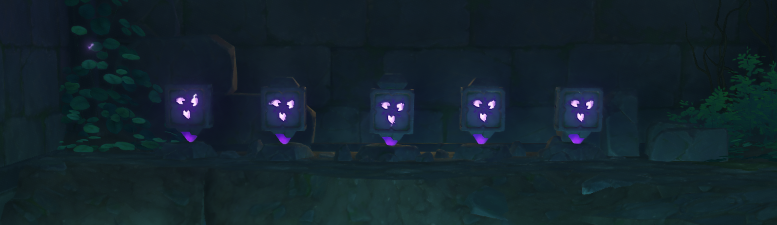
\includegraphics[width=\linewidth]{images/E_1.png}
\end{center}

这个机关上面有 $p$ 个灯,每个雷立方体受到一次攻击时便点亮一个灯,当 $p$ 个灯全部被点亮并受到一次攻击后会熄灭所有的灯。

现在 |Tifa| 面前有 $n$ 个雷立方体,编号为 $1,2, \cdots, n$。|Tifa| 会对其中若干个雷立方体攻击若干次,在这之后 |Tifa| 想知道其中某些雷立方体中哪个点亮的灯最多。

由于 |Tifa| 太菜了,所以他来求助你。又由于 |Tifa| 急着去雪山堆雪人,所以你只有 1.5s 的时间回答 |Tifa| 的问题。

\section*{输入格式}

第一行,两个整数 $n,p~(1 \leq n \leq 2 \times 10^5, 2 \leq p \leq 10^9+7)$, 含义见题目描述。

第二行,$n$ 个整数 $a_1, a_2, \cdots, a_n~(0 \leq a_1, a_2, \cdots, a_n \leq p)$, 表示编号为 $1,2, \cdots, n$ 的雷立方体初始点亮的灯数。

第三行,一个整数 $q,~(1 \leq q \leq 2 \times 10^5)$, 表示操作次数。

接下来 $m$ 行,每行均为且仅为如下格式之一:

\begin{enumerate}
	\item |1 x k|: 攻击 $a_x~k$ 次,$k \geq 0$;
	\item |2 x y|: 输出 $a_x, a_{x+1}, \cdots, a_y$ 间的\textbf{最大值}以及对应的编号,若最大值相同则优先输出编号小的。
\end{enumerate}

注意,如果某次操作不合法, 则应输出 |invalid| 并忽略该次操作。

保证所有输入数据均在 |int| 范围内。

\section*{输出格式}

输出 $m$ 行,每次操作后均需输出一行,其中:

\begin{itemize}
	\item 若操作不合法 (即对于操作 $1$ 不满足 $1 \leq x \leq n$, 对于操作 $2$ 不满足 $1 \leq x \leq y \leq n$), 则输出 |invalid|;
	\item 若为操作 $1$ 且 $1 \leq x \leq n$, 则该行什么也不需要输出;
	\item 若为操作 $2$ 且 $1 \leq x \leq y \leq n$, 则输出结果。
\end{itemize}

\section*{输入输出样例}
\testcasetab
{
	7 114514\par
    1 9 1 9 8 1 0\par
    6\par
    2 1 1\par
    1 5 114511\par
    2 5 7\par
    1 0 1\par
    1 4 114507\par
    2 4 4
}
{
    1 1\par
    \hspace*{\fill} \par
    4 5\par
    invalid\par
    \hspace*{\fill} \par
    1 4
}

\makeproblem
\section*{题目描述}
围棋是一种策略型两人棋类游戏,是我国的非物质文化遗产。围棋使用正方形格状棋盘及黑白二色圆形棋子进行对弈,棋盘上有纵横各 $n$ 条线段将棋盘分成 $n^2$ 个交叉点,棋子必须走在交叉点上,双方交替行棋,落子后不能移动。

我们管棋盘中的每部分连接在一起的棋子叫做一块棋,例如下图中黑棋有 $3$ 块棋,而白棋有 $4$ 块棋。

\begin{center}
	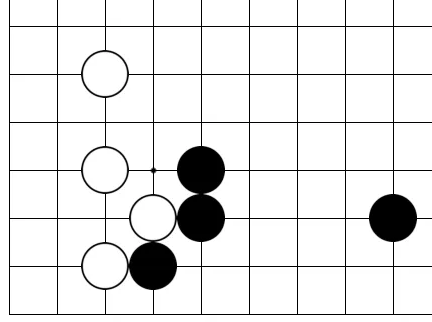
\includegraphics[scale=0.5]{images/go_1.png}
\end{center}

若一着棋落下后,其将本方的若干块\textbf{之前未连接在一起的棋}连接在了一起成为了一块棋,那么这着棋叫做“粘”,例如下图中白 $\Delta$ 子就是一手“粘”:

\begin{center}
	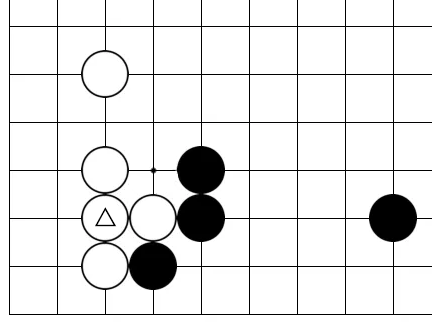
\includegraphics[scale=0.5]{images/go_2.png}
\end{center}

现给出一局围棋的进行过程,请你计算出:

\begin{itemize}
	\item 共有几手棋是“粘”?
	\item 最终局面下黑白双方各有多少块棋?
\end{itemize}

注意:

\begin{itemize}
	\item 黑棋先行;
	\item 为使问题简单,不必考虑“提”的情况;
	\item 所有棋子并不一定全部下完。
\end{itemize}

\section*{输入格式}
第一行,一个整数 $n~(1 \leq n \leq 500)$,代表棋盘的边长。

第二行,一个整数 $c~(1 \leq c \leq n^2)$,代表双方共下了几着棋。

接下来 $c$ 行,每行两个整数 $x,y~(1 \leq x,y \leq n)$,代表一着棋所下的位置。数据保证不会出现重复落子的情况(也就是说数据一定合法)。注意黑白双方是交替行棋的,也就是说奇数行的棋子是黑方下的,偶数行的棋子是白方下的。

\section*{输出格式}
第一行,两个整数,分别代表黑白双方行棋过程中各有几手棋是“粘”。

第二行,两个整数,分别代表黑白双方最终局面下各有多少块棋。

\section*{输入输出样例}
\testcasetab
{
	4\par
	8\par
	2 2\par
	3 3\par
	2 3\par
	1 3\par
	1 1\par
	3 2\par
	3 4\par
	4 4
}
{
	0 1\par
	3 2
}

\end{document}